% !TEX TS-program = pdflatex
% !TEX encoding = UTF-8 Unicode

\documentclass[11pt]{article}
\usepackage[utf8]{inputenc} 
\usepackage[parfill]{parskip}
\usepackage[T1]{fontenc} 

\usepackage{polski}
\usepackage{float}
\usepackage{fixltx2e}
\usepackage{calc}
\usepackage[export]{adjustbox} % also loads graphicx
\usepackage{makeidx}
\usepackage{multicol}
\usepackage{multirow}
\PassOptionsToPackage{warn}{textcomp}
\usepackage{textcomp}
\usepackage[nointegrals]{wasysym}
\usepackage[table]{xcolor}

\usepackage{csvsimple}

% Font selection
\usepackage[T1]{fontenc}
\usepackage[scaled=.90]{helvet}
\usepackage{courier}
\usepackage{amssymb}
\usepackage{sectsty}

%%% PAGE DIMENSIONS
\usepackage{geometry} % to change the page dimensions
\geometry{a4paper} % or letterpaper (US) or a5paper or....
\geometry{margin=1in} % for example, change the margins to 2 inches all round

\usepackage{graphicx} % support the \includegraphics command and options
\usepackage[parfill]{parskip} % Activate to begin paragraphs with an empty line rather than an indent

%%% PACKAGES
\usepackage{booktabs} % for much better looking tables
\usepackage{array} % for better arrays (eg matrices) in maths
\usepackage{paralist} % very flexible & customisable lists (eg. enumerate/itemize, etc.)
\usepackage{verbatim} % adds environment for commenting out blocks of text & for better verbatim
\usepackage{subfig} % make it possible to include more than one captioned figure/table in a single float
% These packages are all incorporated in the memoir class to one degree or another...
\usepackage{graphicx}

\usepackage{ifpdf}
\ifpdf
\usepackage[pdftex,pagebackref=true]{hyperref}
\else
\usepackage[ps2pdf,pagebackref=true]{hyperref}
\fi
\hypersetup{%
	colorlinks=true,%
	urlcolor=blue,
	linkcolor=blue,%
	citecolor=blue,%
	unicode%
}


%%% HEADERS & FOOTERS
\usepackage{fancyhdr} % This should be set AFTER setting up the page geometry
\pagestyle{fancy} % options: empty , plain , fancy
\renewcommand{\headrulewidth}{0pt} % customise the layout...
\lhead{}\chead{}\rhead{}
\lfoot{}\cfoot{\thepage}\rfoot{}
%%% END Article customizations

%%% The "real" document content comes below...

\title{Optymalizacja hiperparametrów xgboost\\
	\large Dokumentacja wstępna}

\author{Przemysław Stawczyk, Piotr Zmyślony}
\date{15 kwietnia 2020} % Activate to display a given date or no date (if empty),
% otherwise the current date is printed 

\begin{document}
	\maketitle
	\setcounter{secnumdepth}{3}
	\setcounter{tocdepth}{3}
	\tableofcontents
	\clearpage

\section{Treść zadania}
Naszym zadaniem jest przetestowanie różnych algorytmów heurystycznych/populacyjnych w kontekście problemu strojenia hiperparametrów algorytmu xgboost. Problem wyboru hiperparametrów wynika z ich bardzo dużej ilości, co często rozwiązane jest poprzez manualny dobór parametrów klasyfikatora.

Projekt zostanie zrealizowany w języku Python 3+.
\section{Dane testowe}
Jako dane na których będziemy trenować i testować klasyfikatory przyjęliśmy proponowany zestaw danych \url{https://www.kaggle.com/c/porto-seguro-safe-driver-prediction}. Zawiera on 57 atrybutów opisujących klientów firmy ubezpieczeniowej i jeden atrybut binarny sygnalizujący, czy w ciągu roku od zawarcia umowy, klient skorzystał z ubezpieczenia.

\begin{figure}[H]
	\caption{Brakujące atrybuty}
	\label{attrib_analysis}
	\centering
	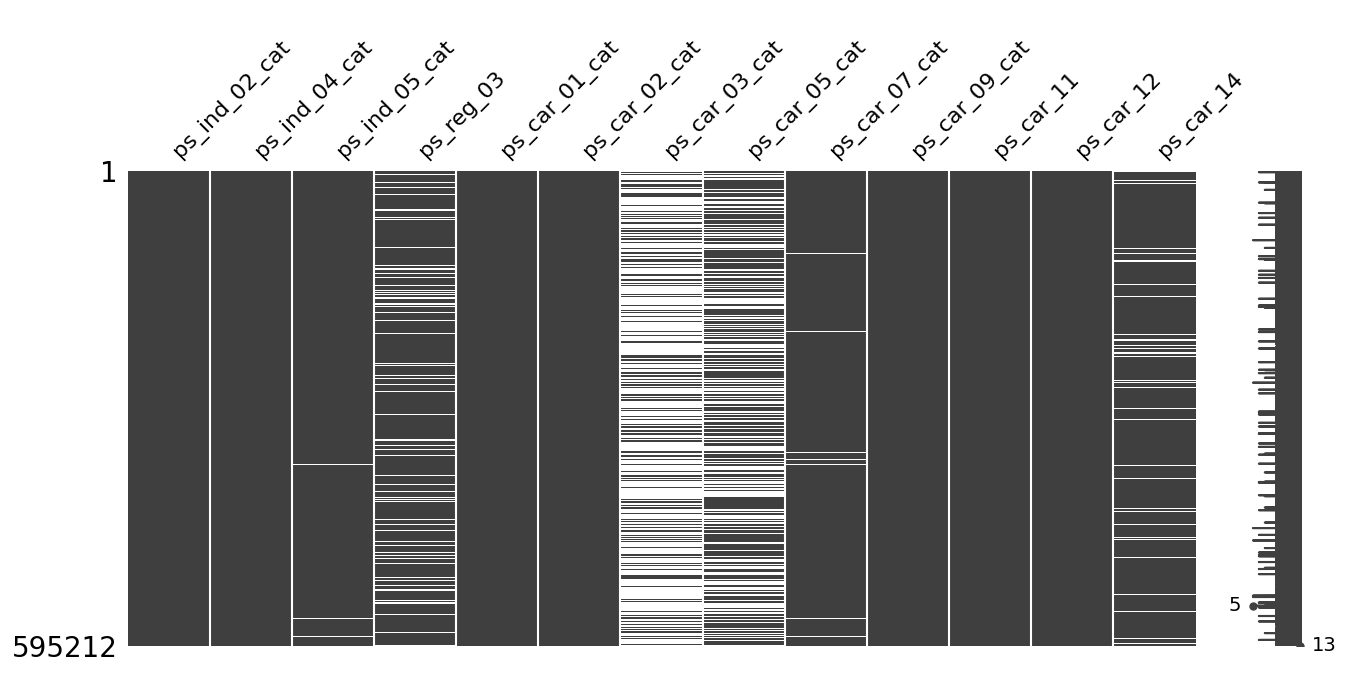
\includegraphics[width=\textwidth]{attrib_analysis}
\end{figure}

\subsection{Analiza danych}
Po wstępnej analizie danych odkryliśmy, że w zbiorze danych posiadamy około 79\% niekompletnych wierszy. Rysunek \ref{attrib_analysis} przedstawia pokrycie niekompletnych atrybutów - jest ich jedynie 13, z czego większość jest wybrakowana w bardzo niewielkim stopniu.

Największym winowajcą jest atrybut binarny \textsl{ps\_car\_03\_cat}, którego brakuje aż w 70\% wierszy, oraz atrybut \textsl{ps\_car\_05\_cat} (brakuje go w 44\% przypadków). W końcowej wersji zdecydowaliśmy się usunąć oba z tych parametrów.

Dodatkowo, występuje znaczna dysproporcja między klasami rekordów - tylko 3\% wierszy opisuje klientów, którzy skorzystali z ubezpieczenia. Stąd niezbędna będzie interpolacja danych, tak aby ilość rekordów obu klas była równa.

\section{Algorytmy}
Zaimplementowaliśmy następujące algorytmy:
\begin{itemize}
	\item algorytm wspinaczkowy z tabu. \\ 
	W 2 wariantach:
		\begin{itemize}
			\item mutacyjny z prawdopodobieństwem P mutacji jednego (losowego) z parametrów
			\item z przeglądem sąsiedztwa i powracaniem
		\end{itemize}
	\item przegląd wyczerpujący hipersiatki jako metoda bazowa\\
\end{itemize}

W przypadku mutacji połączonej z tabu, problematycznym okazało się tworzenie mutantów z wykorzystaniem rozkładu normalnego, jak i mutacji w ten sam sposób wielu parametrów - tworzone były wielokrotnie już sprawdzone zestawy parametrów.\\\\
Przyjeliśmy metodę w której tworzone są wszystkie (jeszcze niezbadane) możliwe zestawy różniące się jednym parametrem w stosunku do rodzica i spośród nich losowany jest nowy mutant.

\subsection{Przestrzeń poszukiwań}
Trenowane modele posiadały parametry z hipersiatki, czyli iloczyn zbiorów każdego z parametrów, co w sumie daje nam 52272 dopuszczalnych rozwiązań.
\begin{center}
	\begin{tabular}{|c|c|}
		\hline
		nazwa parametu & zakres \\
		\hline
		\hline
		liczba słabych modeli &  50, 75, 100 ... 300\\ % 0.3 = default
		\hline
		eta &  0.1, 0.2, 0.3, 0.4\\ % 0.3 = default
		\hline 
		min\_split\_loss \textit{gamma} & 0, 1, 2, 3\\ % 20 = extremly high
		\hline 
		max\_depth & 4, 5, 6 ... 14\\
		\hline 
		max\_delta\_step & 0, 1, 2\\
		\hline 
		subsample & 0.6, 0.8, 1\\
		\hline
		colsample\_bytree &  0.6, 0.8, 1\\ % 1 = default
		\hline 
	\end{tabular}
\end{center}

Dalej, \textit{sąsiadem} zestawu A będziemy nazywali takie zestawy parametrów, które od zestawu A różnią się tylko jednym parametrem, większym bądź mniejszym o jeden "kwant".

\subsection{Funkcja celu}
Jako funkcję celu przybraliśmy \textit{Average Precision Recall} obliczając wartość funkcji celu jako średnią arytmetyczną skuteczności przypisania predykcji. Zastosowaliśmy implementację z pakietu \textit{scikit-learn}.\\
Ta sama funkcja zostanie wykorzystana do oceny jakości finalnych wytrenowanych modeli na zbiorach testowych, przy 3-krotnej walidacji krzyżowej, gdzie nasz końcowy jest średnią osiągniętych wyników AUC ROC.

\subsection{Algorytm brutalny}
Algorytm brutalny generuje zbiór wszystkich możliwych zestawów parametrów, które przegląda krok po kroku. Wynikiem działania jest zestaw parametrów osiągający najwyższy wynik AUC ROC.

\subsection{Algorytm wspinaczkowy}
Jako parametr startowy algorytmu należy podać maksymalną ilość powrotów \texttt{n\_max}, które może wykonać przed zwróceniem aktualnego najlepszego wyniku. Zaczyna swoje działanie od wylosowania punktu startowego z dostępnych zbiorów parametrów (na początku przypisujemy go do \texttt{P\_b} i \texttt{P\_c}). Oblicza wynik dla \texttt{P\_c} dalej w następujący sposób:
\texttt{
\begin{enumerate}
\item Ustaw liczbę nawrotów n = 0
\item Jeśli n > n\_max, przejdź do punktu ostatniego.
\item Wygeneruj wszystkich (nigdy nieodwiedzonych) sąsiadów P\_c.
\item Wybierz sąsiada, który daje wynik lepszy bądź równy wynikowi P\_c.
\item Jeśli nie istnieje taki sąsiad:
	\begin{enumerate}
	\item n = n + 1
	\item ustaw P\_c na poprzedni P\_c
	\end{enumerate}
\item Jeżeli istnieje:
	\begin{enumerate}
	\item n = 0
	\item P\_c = najlepszy sąsiad
	\item Jeżeli wynik P\_c >= P\_b: P\_b = P\_c
	\end{enumerate}
\item Wróć do punktu 2.
\item Zwróć najlepszy zestaw parametrów.
\end{enumerate}
}






\section{Sposób mierzenia jakości rozwiązania}
Jako że trenowanie znacznej liczby modeli przy użyciu adekwatnych ilości danych wejściowych jest bardzo czasochłonne, postanowiliśmy zaimplementować opcję testowania wszystkich trzech algorytmów w określonych ramach czasowych. Dzięki podaniu odpowiedniego parametru, program uruchamia każdy z nich tylko na jakiś czas, po którym algorytm musi zwrócić najlepszy dotychczasowy wynik.

Wszystkie opcje uruchomieniowe programu można sprawdzić poleceniem:

 \texttt{python performance\_test.py -\--help}
%Będziemy porównywać algorytm pod kątem czasu działania względem wyczerpującego przeglądu, analizując czy zysk z szybszego doboru parametrów jest wystarczająco duży, by go stosować dla różnych limitów przejrzanych kombinacji dla naszych algorytmów.
%\\
%Zbiór danych zostanie podzielony na 2 podzbiory - uczenia i testowy \textsl{uczący odpowiednio większy}. Na zbiorze testowym nie będziemy uczyć i podejmować decyzji - zostanie on wykorzystany do zmierzenia działania algorytmu po dobraniu wszystkich parametrów. Zbiór uczący będzie działać z k-krotną walidacją krzyżową lub podzielony na zbiór uczenia i weryfikacyjny.

\section{Wyniki pomiarów}
Otrzymane rezultaty dla algorytmu wspinaczkowego i algorytmu mutacyjnego są oddalone od siebie nieznacznie, ale różnice możemy zaobserwować w przebiegu ich działania. Poniższe wykresy reprezentują wszystkie zestawy parametrów, które pobiły dotychczasowy najlepszy wynik.
\begin{figure}[H]
	\caption{Wykres najlepszego dotychczasowego wyniku w zależności od czasu}
	\label{nice_mutation}
	\centering
	\includegraphics[scale=0.85]{nice_mutation}
\end{figure}
Na wykresie, około 50. sekundy możemy zaobserwować taką mutację zestawu parametrów, która dała znaczny wzrost AUC ROC, a potem wyraźny jest proces znajdywania przez algorytm lokalnego optimum.


\section{Wnioski i rekomendacje}
% tak serio to trzeba napisać coś XDDDD
Algorytmy zbytnio nie były efektywne \textit{imho} należałoby walnąc se parę paramsów i okolice obiecujących zbadać przegłądem wyczerpującym Xd

\end{document}